\section{JavaScript}
\label{js}

JavaScript ist eine Programmiersprache/Skriptsprache, die üblicherweise in Webseiten Verwendung findet. Sie wird jedoch auch noch vielen Umgebungen außerhalb der Website Entwicklung benutzt, 
wie zum Beispiel \nameref{nodejs}.
JavaScript besitzt First-Class-Funktions (Funktion erster Klasse). Außerdem is JS eine prototypbasierte Sprache, welche mehreren Paradigmen folgt, dynamisch ist und sowohl 
objektorientiert als auch deklarative Programmierung ermöglicht. JavaScript ist plattformunabhängig.

\subsection{First-Class-Funktions}
Funktionen erster Klasse werden wie Variablen behandelt. Bei einer Programmiersprache welche First-Class-Funktionen besitzt, kann man Funktionen als Parameter übergeben, einer Variable zuweisen oder
einer anderen Funktion zurückgegeben werden.
\pagebreak

\begin{center}
    \subsubsection{Beispiel für die Zuweisung einer Funktion an eine Variable}
\begin{figure}[htbp]
    \centerline{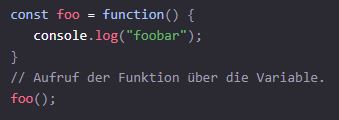
\includegraphics{Theorie/JavaScript/Funktion-in-Variable.png}}
    \caption{Zuweisung einer Funktion an eine Variable.~\cite{First-Class-Funktion}}
\end{figure}
\end{center}
Hier wird der Variable \textit{foo} eine anonyme Funktion zugewiesen, welche und in der Konsole eine Ausgaben liefert.
Diese Funktion wird dann ganz einfach über die Variable mittels den zwei Klammern aufgerufen.


\begin{center}
    \subsubsection{Beispiel für das Übergeben einer Funktion als Argument}
\begin{figure}[htbp]
    \centerline{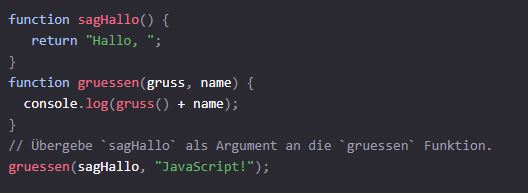
\includegraphics{Theorie/JavaScript/Funktion-als-Argument.png}}
    \caption{Übergeben einer Funktion als Argument.~\cite{First-Class-Funktion}}
\end{figure}
\end{center}
Hier übergeben wird er Funktion \textit{gruessen} 2 Parameter. Als einer dieser beiden Parameter übergeben wir die Funktion \textit{sagHallo} welche ``Hallo, `` als return liefert.
Führen wir nun die Methode gruessen mit diesen Parametern aus, wird in die Console der Satz \textit{``Hallo, Javascript``} geschrieben.
\pagebreak

\begin{center}
    \subsubsection{Eine Funktion als Return}
\begin{figure}[htbp]
    \centerline{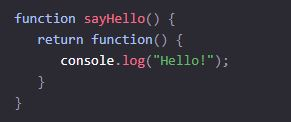
\includegraphics{Theorie/JavaScript/Funktion-als-Return.png}}
    \caption{Funktion als Return.~\cite{First-Class-Funktion}}
\end{figure}
\end{center}
Hier wird ganz einfach als return Wert eine Funktion übergeben.


\subsection{Objektorientierte Programmierung}






